\documentclass[12pt,letterpaper]{article}
\usepackage{graphicx}
\usepackage{multirow}
\usepackage{authblk}
\usepackage{float}
\usepackage{rotating}
\usepackage{url}
\usepackage{lscape}
\usepackage{longtable}
\usepackage{subfigure}
\usepackage{natbib}
\usepackage{lineno}
\usepackage{amsmath,amsthm}
%\usepackage{fullpage}	
\usepackage{anysize}
\marginsize{1.0in}{1.0in}{1.0in}{1.0in}
\linespread{1.6}

\newcommand{\Pic}[2][0.85]{\begin{center}\includegraphics[width=0.8\textwidth,height=#1\textheight,keepaspectratio]{#2}
 \end{center} }


\title{A novel decimation/interpolation technique for gridded surfaces}
\author[1]{ E. R. Stefanescu}
\author[2]{K. Marcus}
\author[1]{A.K. Patra}
\author[3]{M. Bursik}
\affil[1]{Department of Mechanical and Aerospace Engineering, University at Buffalo, Buffalo, NY 14260}
\affil[2]{Department of Computer Science and Engineering, University at Buffalo, Buffalo, NY 14260 }
\affil[3]{Department of Geology, University at Buffalo, Buffalo, NY 14260 }


\date{\today}


\begin{document}
\linenumbers
\maketitle

\begin{abstract}
to be added
\end{abstract}

\section{Introduction}
Digital elevation models have been used in many applications since they came into use in the late 1950s. DEMs are extensively used in geologic mapping, civil engineering, landscape planning, visibility analysis, hydrology and geophysical modeling and are critical to many natural hazard risk applications.
Different applications require different levels of accuracy from digital elevation models. In this study, the magnitudes and spatial patterning of elevation errors were therefore examined, using a novel interpolation methods. Previous research has demonstrated the effects of interpolation methods and the nature of errors in digital elevation models obtained with indirect survey methods for small-scale areas. The main idea of the method comes from the area of dimensionality reduction, where a weighted graph associated with the DEM points it is created.

Dimensionality reduction occupies a central position in many fields such as information theory, where it is related to compression and coding, statistics, with latent variables, as well as machine learning and sampling theory. In essence, the goal is to change the representation of data sets, originally in a form involving a large number of variables, into a low-dimensional description using only a small number of free parameters. The new representation should describe the data in a faithful manner, preserving some quantities of interest such as local mutual distances. Analogous to the problem of dimensionality reduction is that of finding meaningful structures in data sets. The goal here is to extract relevant features out of the data in order to gain insight and understanding of the phenomenon that generated the data.

In order to achieve any of these two goals, numerous data mining and machine learning techniques rely on graph-based algorithms. In terms of data structures, graphs offer an advantageous compromise between their simplicity, interpretability and their ability to represent complex relationship between data points. Weighted graphs are usually employed to represent a notion of geometry based on the local similarity or interactions between data points. In many situations, each data sample is represented by a collection of numerical attributes, and in this case, the condition for two nodes to be connected is based on the proximity of the corresponding data point in the feature space.

Graph, directed or undirected, are important modeling objects in many modern applications: 1) data clustering, via building a pairwise similarity graph by which the clustering problem is naturally transformed to a graph partitioning problem; 2) analysis of online social networks; 3) visual object recognition; 3) analysis of complex networks from biological networks; 4) image segmentation, etc. In all of these applications the edges of the graphs represent connections or relations or links between vertices. The vertices could be interacting users, genes or pixels in a image.

Since 1995, multilevel algorithms have become a popular approach for graph partitioning. This class of algorithms recursively reduces the size of the graph (i.e., coarsens the graph) by collapsing vertices and edges, partitions the smallest (coarsest) one and then uncoarsens it to construct partitions of all subsequent larger graphs until a partition for the original graph is obtained. The coarsening process is based on matching nodes according to some heuristics (e.g., heavy edge matching). The matched nodes are ``collapsed" (merged) to create a new multinode with a volume equal to the sum of their volume. Similarly the edges connecting multinodes are the sum of the edges incident on the corresponding matched nodes. The coarsest level (smallest graph) is then partitioned by various heuristics. During the uncoarsening (interpolation) process the matched nodes are simply separated and each gets the partition of its multinode. 

General multilevel techniques have been successfully applied to various areas of science (e.g., physics, chemistry, engineering, etc.). Multigrid methods are very efficient iterative solvers for system of algebraic equations arising from finite element and finite difference discretizations of partial differential equations. The main principle of multigrid methods is to complement the local exchange of information in point-wise iterative methods by a global one utilizing several related systems, called ``coarse level", with a smaller number of variables.
The name multigrid comes from the fact that the original algorithms were based on a nested grid hierarchy, with intergrid transfer operators based on the geometry of these grids. For this reason, these classical multigrid algorithms are often referred to as geometric multigrid methods. While these methods perform well for PDEs with smooth coefficients, it has been observed 
that performance of classical, geometric multigrid methods breaks down when there is significant variation in the coefficient of the PDEs. 

Given a DEM, we first construct a graph so that every points is a node in the graph and neighboring points are connected by an arc.


\section{Multigrid}

\subsection{Geometric Multigirid}

\subsection{Algebraic Multigrid}

\section{Weighted Aggregation clustering}
In the context of graphs it is the Laplacian matrix that represents the related sets of equations attached to a graph. The main difference between the AMG approach and other multilevel ones is the coarsening scheme. While the latter may be viewed as a strict aggregation process, the AMG coarsening is actually a weighted aggregation: each node is divided into fractions, and different fractions belong to different aggregates (multimodes). In both cases, these aggregates will form the nodes of the coarser level. 

The disaggregation consists projecting to a finer level the final partition obtained at the next coarser level. This initial fine level partition is being further improved by applying local processing first of strict minimization. 


\section{Multiscale sampling}

\subsection{Randomized algorithms}
We are concerned with the fundamental problem of approximately factorizing an arbitrary $m\times n$ matrix A as
\begin{align}
A_{m \times n} \approx B_{m\times k} C_{k\times n} 
\end{align}
where $k \le \min(m,n)$ is the desired rank. The goal is to compute $B$ and $C$ such that $A -BC$ is as small as possible. The 
quality of the approximation is measured by taking either the spectral norm $\parallel \cdot \parallel$ ($l^2$- operator, equivalent 
with the largest singular value) or the Frobenius norm $\parallel \cdot \parallel_F$ ( the root-sum of squares of the singular values) of
the residual $A - BC$. 
The best rank-$l$ approximation, measured either in the spectral or Frobenius norm, is obtained by truncating the singular value
decomposition (SVD)
\begin{align}
\parallel A - U\Sigma V^T\parallel \le \delta
\end{align}
with $U$ being a $m \times k$ matrix whose columns are orthonormal, $V$ being an $n \times k$ matrix whose columns are orthonormal,
and $\sigma$ being a diagonal $k \times k$ matrix whose entries are all nonnegative. 

\subsection{Random projection}

\subsection{Implementation}
Almost any method one can think of in data analysis and scientific computing relies on matrix algorithms. In the era of ``big data", we must now routinely deal with matrices of enormous sizes and reliable algorithmic solutions for computing solutions to least-squares problems, for computing approximate QR and SVD factorizations and other such fundamental decompositions are urgently needed. The development of randomized algorithms for numerical linear algebra has
seen a new surge in recent years, providing powerful tools for constructing approximate matrix factorization. These techniques are simple and effective. 

In many machine learning and data analysis applications, one is interested in symmetric positive semi-definite (SPSD) matrices, e.g., kernel matrices and Laplacian matrices. One common column-sampling-based approach to low-rank approximation of SPSD matrices is the Nystr\"{o}m method. The simplest Nystr\"{o}m-based procedure selects columns from the original data set uniformly at random and then uses those columns to construct a low-rank SPSD approximation.  Although this procedure can be effective in practice for certain input matrices, there are two extensions to the method that can substantially improve the performance, e.g. lead to lower reconstruction error for a fixed number of column samples, both in theory and practice.  The first extension is to sample columns with a nonuniform importance sampling distribution; and then the second extension is to randomly mix (or combine linearly) columns before sampling them. For the random sampling algorithm, an important question is what importance sampling distribution should be used construct the sample; while for the random projection algorithms, an important question is how to implement the random projections. In either case, appropriate consideration should be paid to questions such as whether the data are sparse or dense, how the eigenvalue spectrum decay, the nonuniformity properties of eigenvectors, and so on.  
A combination of clustering and a low-dimensional rank approximation gives a much better approximation of the original graph. In particular, information from every cluster is extracted regardless of their relative sizes.  Different clusters of graphs have distinct meanings and are usually of varying sizes. A standard low rank computation is likely to only extract information from the largest or a few dominant clusters, thus filtering out smaller ones completely. 

Theoretically, the optimal low-rank approximation (w.r.t spectral or Frobenius norm) of a given matrix can be provided by standard matrix decomposition such as QR and SVD. However, finding such optimal low-rank approximation is not always feasible, especially in the case of large-scale problem.  For example, the complexity of SVD is $\mathcal{O}(m^3)$ for an $m\times m$ matrix $A$. Comparing with them the low-rank approximation algorithms provide lower time complexity $\mathcal{O}(km^2)$ and can be accelerated to $\mathcal{O}(\log (k)m^2)$, where $k$ is the target rank. 

In the analysis of large scale simulations of complex dynamical systems, where the notion of time evolution comes into play, important problems 
are the identification of variables that capture the time evolution of the system. Traditionally, creating hazard maps has required detailed knowledge 
of past events which has been recorded in the volcano's geologic record. Knowledge of this history is frequently incomplete or even entirely unavailable.
Our goal is to produce a map showing the probability that each East-North point has of being inundated by a volcanic landslide with a flow-depth greater than a critical threshold from a collection of simulator runs whose parameters are drawn from a distribution that represents a volcanologist's best guess of the range of possible scenarios. We consider a study case for Soufri\`ere Hills, Montserrat, for which ranges of the flow volume, bed friction, internal friction and direction are available.
The 4-dimensional input parameter space is sampled using a simple space filling design like Latin Hypercube Design (LHD) to obtain 2048 sets of input. Simulations are performed at each sample point using the TITAN2D model to generate a map of maximum pile height, $h_{max}(\textbf{x})$ as function of position.
By performing a multiscale data sampling we identify a well-conditioned basis of a low rank Gaussian kernel matrix, used in identifying scattered data sampling (Fig.~\ref{fig_lhs} - red stars). Using the obtained sample data, $h_{max}$ is evaluated at re-sample points.

Typical usage involves evaluating the fast surrogate at hundreds of thousands or millions of re-sample input points. The number of samples needed to generate the fast surrogate are exponential in the number of dimensions. This effectively limits its application to when there are three or fewer uncertain dimensions. This implies that we need to change the representation of the 2048 data sets, into a low-dimensional that describe the data in a faithful manner. In order to achieve this goal, we use a technique that relies on graph-based algorithms. Weighted graphs are employed to represent the ``geometry" based on the local similarity or interaction between the data points. Since each of the data sample is represented by a collection of numerical attributes, the condition of two nodes to be connected is based on the proximity of the corresponding data points in the feature space.

A graph $G=(V,E)$ is characterized by a set of vertices $V=\{1,\dots,m\}$ and a set of edges $E=\{e_{ij}|i,j \in V\}$.
Let $A=[a_{ij}]$ be the $m\times m$ adjacency matrix such that $a_{ij}$ represents the weight of edge $e_{ij}$. If there is no edge between vertices $i$ and $j$ then $a_{ij}=0$.
Clustering the vertices $V$ into $c$ disjoints sets $V_1, \dots, V_c$ with $m_i=|V_i|$, the adjacency matrix will have
the following form:
\begin{equation}
A_{m,n} =
 \begin{bmatrix}
  A_{11}  & \cdots & A_{1c} \\
  A_{2,1} & \cdots & A_{2,n} \\
  \vdots  & \ddots & \vdots  \\
  A_{c1}  & \cdots & A_{c,c}
 \end{bmatrix}
\end{equation}
where each diagonal block $A_{ii}, i=1,\dots,c$, is an $m_i \times m_i$ matrix that can be considered as a local
adjacency matrix for cluster $i$. The off-diagonal $m_i \times m_j$ blocks $A_{ij}$ with $i \neq j$, contain the
set of edges between vertices belonging to different clusters.

In a perfectly clusterable graphs, the off-diagonal blocks will not contain any edges, thus yielding $A_{ij}=0$,
and the graph will consist of $c$ disconnected components. In a realistic scenario, with a graph forming good clusters
most of the edges will be contained within the diagonal blocks $A_{ii}$, while the off-diagonal blocks $A_{ij}$ will
contain only a few edges.
The decay in the $A$'s spectrum is a measure of the connectivity of the points in the graph.
\begin{itemize}
\item One extreme case corresponds to the graph where all the all the nodes are disconnected. This leads to
$A$ being equal to the identity operator and thus to a flat spectrum.
\item Another case is the graph where all the nodes are connected to all the other nodes weights equal to
$1$. In this case, $A$ has one eigenvalue equal to 1, and all other eigenvalues are equal to 0 (we obtain the
fastest decay possible for the a diffusion operator).
\item Usually the spectrum of the heat kernel decays smoothly. 
\end{itemize}

Many dimensionality reduction methods involve a spectral decomposition of large matrices, whose dimensions are proportional to the size of the data, has high computational cost. The $n$ observations
${f_1,f_2,\dots, f_3}$ are considered the data points.
When the covariance of the data points is unknown, an artificial function has to be chose. A Gaussian covariance is a popular choice:
\begin{align}
g_{\epsilon}(x,x') = exp(- \parallel x-x' \parallel ^ 2 / \epsilon)
\end{align}
where $\parallel\dots\parallel$ constitutes a metric on the space (Euclidean distance in our case). The corresponding covariance (affinities) is
\begin{align}
(G_{\epsilon})=g_{\epsilon}(x_i,x_j), \; i,j=1,2,\dots,n.
\end{align}
The combination of clustering and low rank approximation gives a better approximation of the original graph. A standard low rank computation is likely to only extract information from the
largest or a few dominant clusters. 
The $Nystr\ddot{o}m$ method, vastly used for out-of-sample extension has three significant disadvantages: (a) Diagonalization of $G$ costs $\mathcal{O}(n^3)$ operations; (b) $G$ may be 
ill-conditioned due to fast decay of its spectrum, and (c) it is unclear how to choose the length parameter $\epsilon$ since the output is sensitive to the choice of $\epsilon$.
To overcome these limitations a multiscale approach is used: a sequence of Gaussian kernel matrices $G_s, s=0,1, \dots$, whose entries are $(G_{\epsilon})=g_{\epsilon}(x_i,x_j)$, where 
$\epsilon_s$ is a positive monotonic decreasing function of $s$, which tends to zero as the scale parameter $s$ tends to infinity (i.e. $\epsilon_s=2^{-s}$, $s=0,1,\dots$.). 

By the application of a randomized interpolative decomposition(ID) to $G_s$, a well-conditioned basis is identified for it numerical range. In each scale $f$ is decomposed into a sum of its 
projections on this basis and it is extended as $\bar{f}_{*} = G_{*}G^{-1}f$. In addition, selection of the proper columns in $G_s$ is equivalent to data sampling of the associated data points.

The method requires no grid. It automatically generates a sequence of adaptive grids according to the data distribution. It is based on the mutual distances between the data points and on a continuous 
extension of Gaussian functions. In addition, most of the costly computations are done just once during the process, independently of the number of the extended data points since they depend only in the data and on the given function. 
 

\begin{figure}[h!]
\centering
\subfigure[120m DEM]{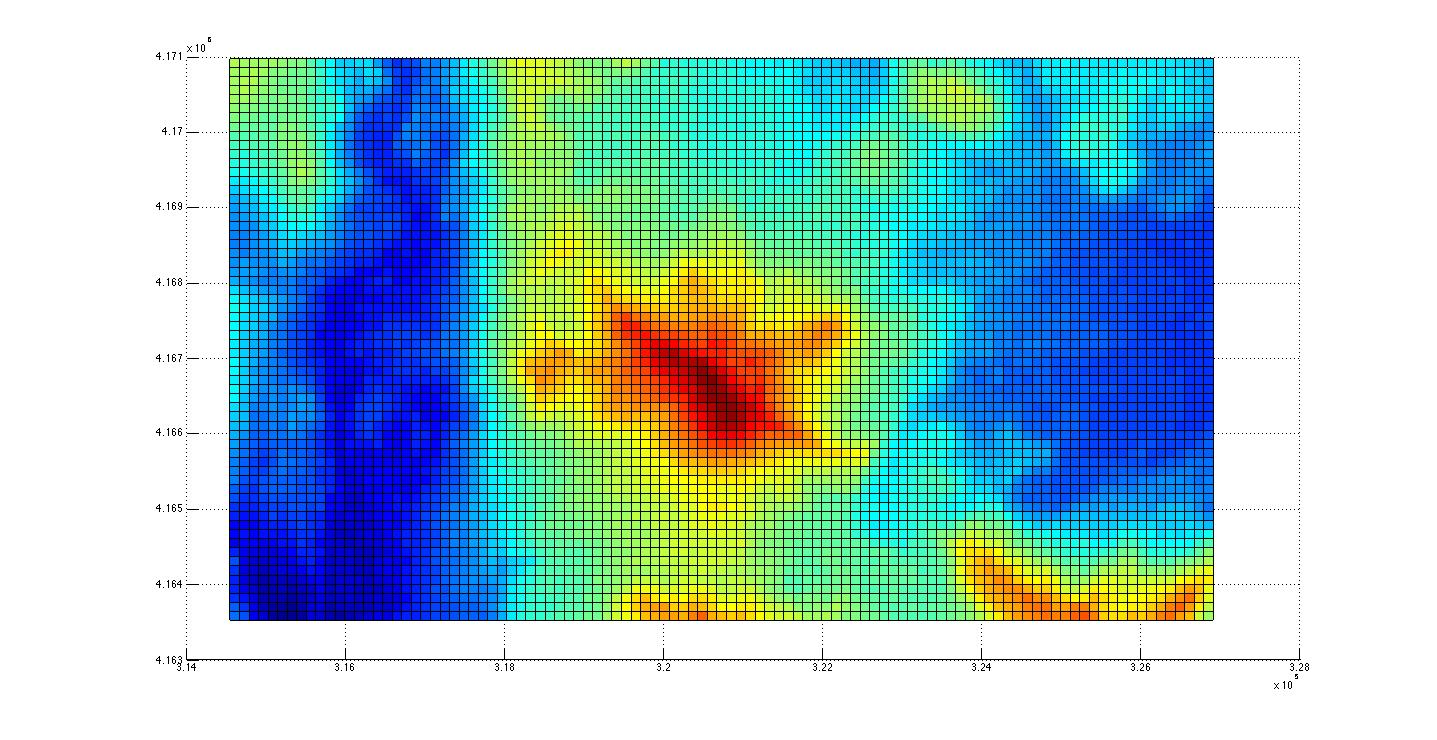
\includegraphics[width=2.8in]{figs/120mDEM.jpg}\label{vrad}}\\
\subfigure[26 sample points]{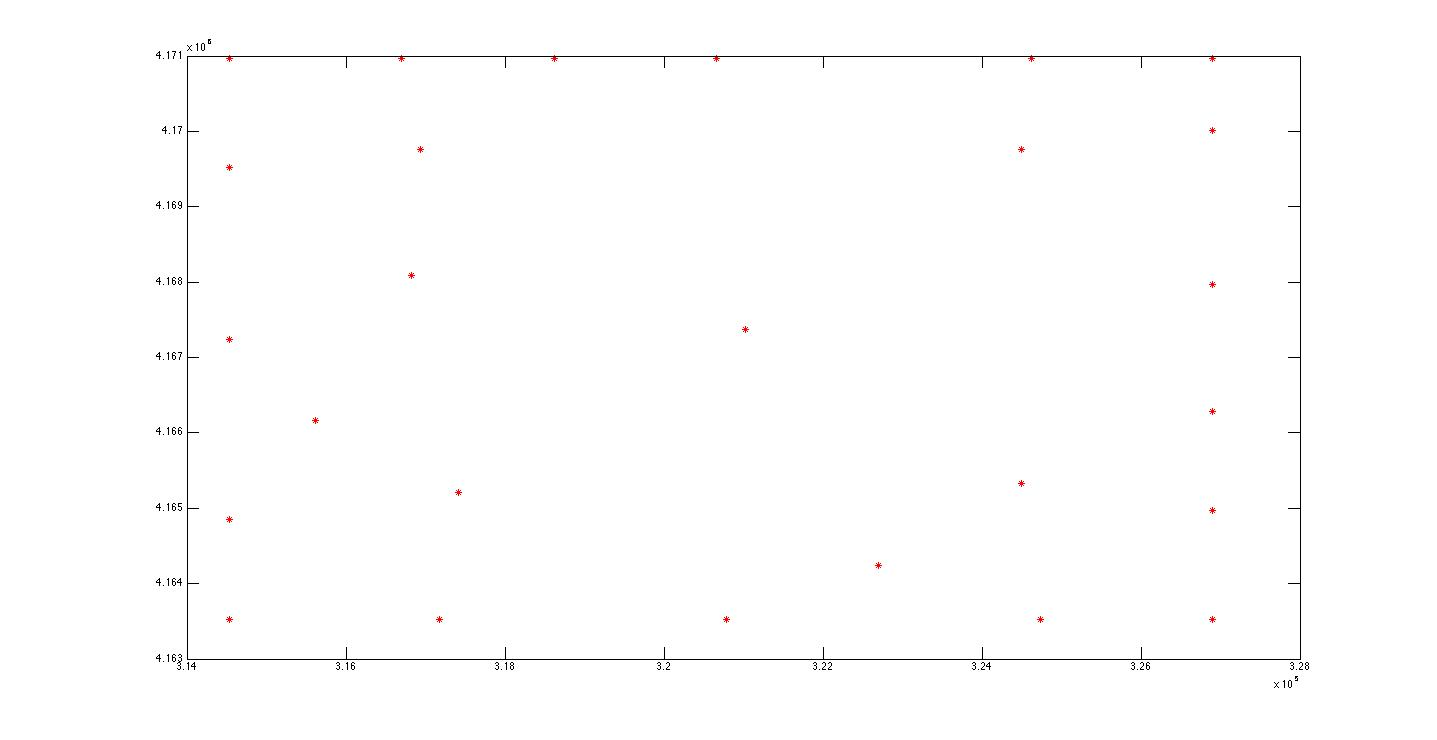
\includegraphics[width=2.8in]{figs/sample_points}\label{vvel}}
\subfigure[]{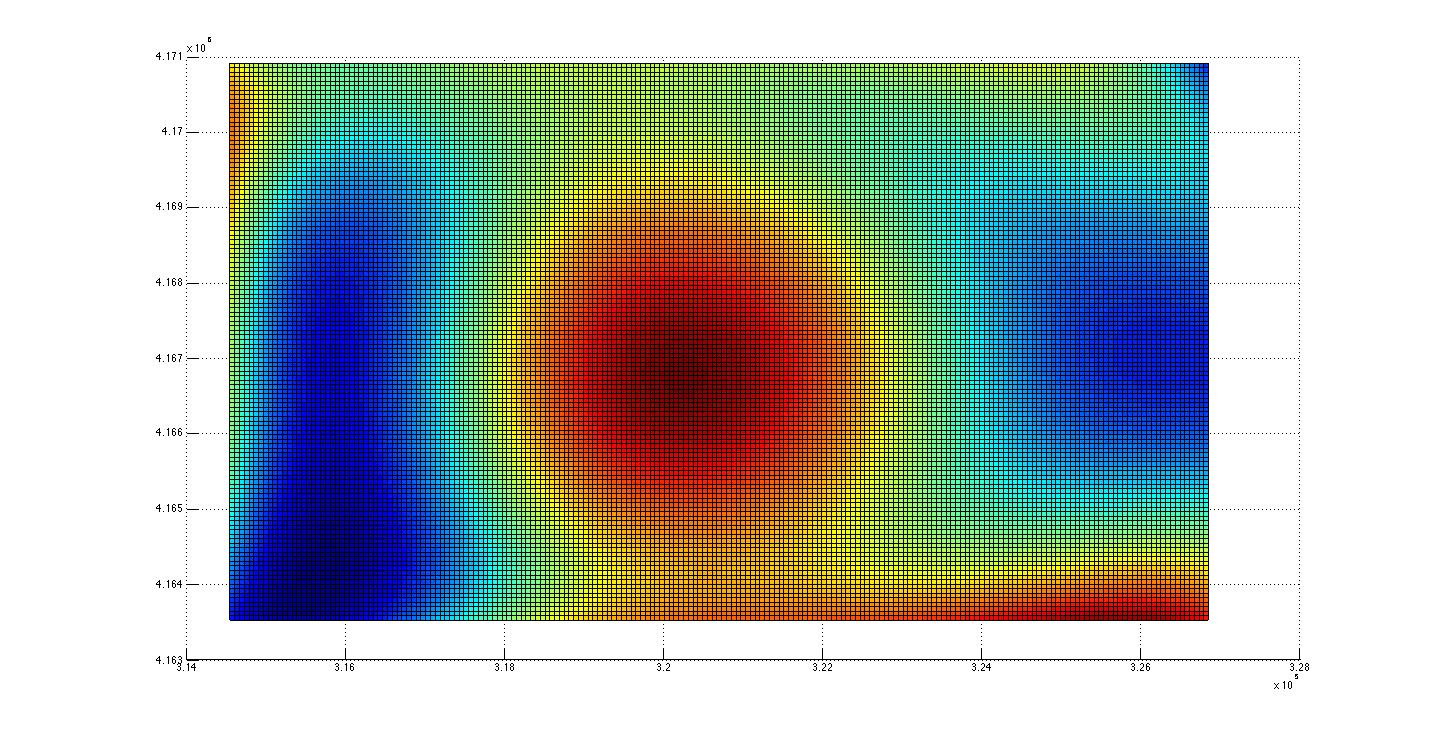
\includegraphics[width=2.8in]{figs/60mDEM_26points}\label{vsize}}
\subfigure[]{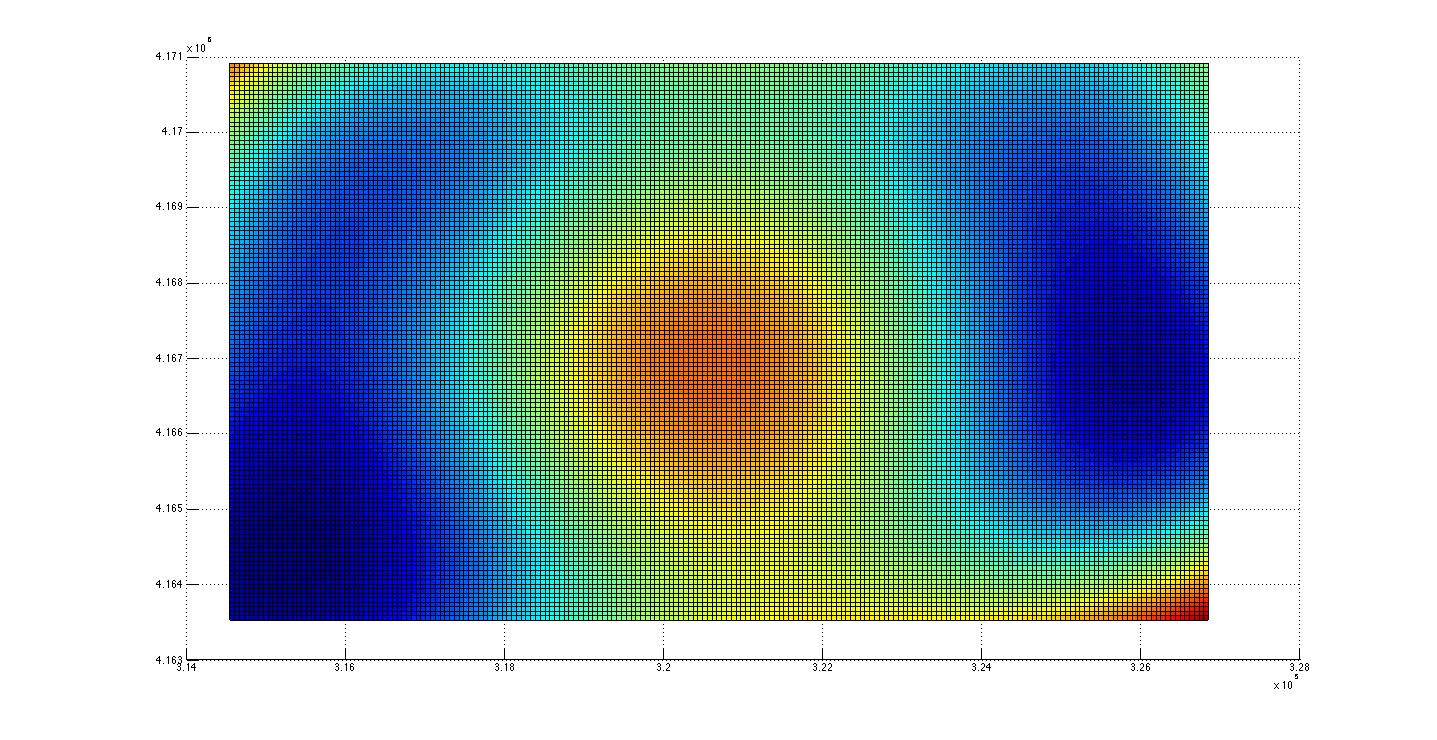
\includegraphics[width=2.8in]{figs/60mDEM_64points}\label{vsigma}}
\subfigure[]{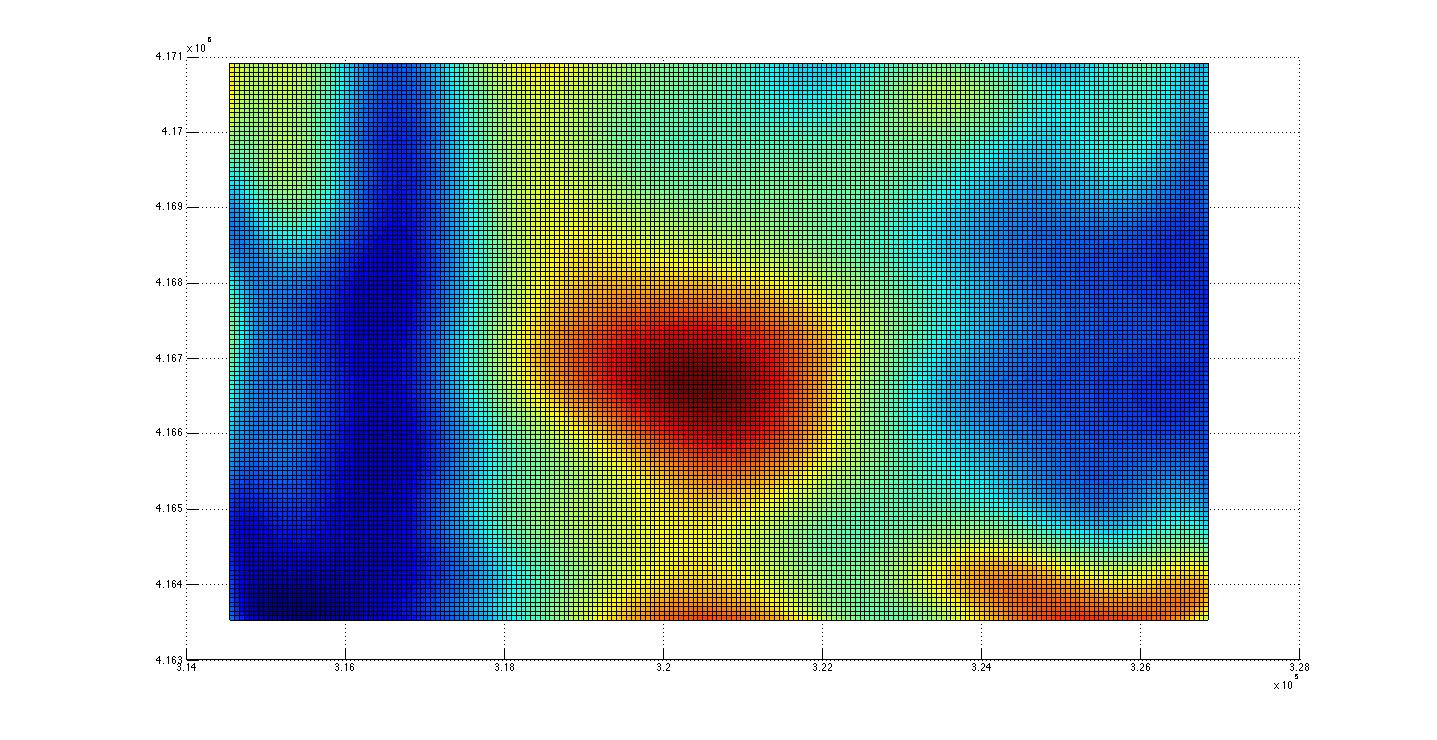
\includegraphics[width=2.8in]{figs/60mDEM_140points}\label{vsigma}}
\caption{DEM high resolution interpolation}\label{src_params_pdf}
\end{figure}

\bibliographystyle{plainnat} \bibliography{mybib}
\end{document}